\documentclass[a4paper,10pt]{report}
\usepackage[T1]{fontenc}
\usepackage[table]{xcolor}
\usepackage{titlesec}
\usepackage{graphicx}
\usepackage[inkscapepath=../assets/svg]{svg}
\usepackage{amsmath}
\usepackage{amsthm}
\usepackage{mathtools}
\usepackage{fancyvrb}
\usepackage[english]{babel}
\usepackage{csquotes}
\usepackage{verbatim}
\usepackage{hyperref}
\hypersetup{
   colorlinks=true,
   linkcolor=blue,
   urlcolor=cyan
}
\usepackage{tikz}
\usepackage{amssymb}
\usepackage[sc]{mathpazo}
\linespread{1.05}
\usepackage{microtype}
\usepackage{breqn}
\usepackage{caption}
\usepackage{subcaption}
\usepackage[
   backend=bibtex,%
   bibencoding=utf8,%
   language=english,%
   style=numeric-comp,%
   sorting=nyt,%
   maxbibnames=10,%
   natbib=true%
]{biblatex}
\addbibresource{references.bib}
\usepackage{siunitx}
\usepackage{booktabs}
\usepackage{longtable}
\usepackage{geometry}
\usepackage{multirow}
\graphicspath{ {../assets/img/} }

\newgeometry{hmargin={30mm,30mm}}

% Set TOC depth and sections numbering
\setcounter{tocdepth}{3}
\setcounter{secnumdepth}{3}

% Remove chapters head and reduce spacing
\titleformat{\chapter}[hang]{\Large\bfseries}{\thechapter \hspace{2ex}}{0pt}{\Large}
\titlespacing{\chapter}{0cm}{0cm}{0.5cm}
\usepackage[parfill]{parskip}

% Make quotes italic
\renewcommand{\mkbegdispquote}[2]{\itshape}

% Change texttt line breaks
\renewcommand{\texttt}[1]{%
  \begingroup
  \ttfamily
  \begingroup\lccode`~=`.\lowercase{\endgroup\def~}{.\discretionary{}{}{}}%
  \catcode`/=\active\catcode`[=\active\catcode`.=\active
  \scantokens{#1\noexpand}%
  \endgroup
}

\usepackage{amsmath}
\newcommand{\argmin}{\mathop{\mathrm{argmin}}}  

\begin{document}
\frenchspacing

% First page
\title{
  {{\large{\textsc{Alma Mater Studiorum $\cdot$ University of Bologna}}}}
  \rule{\textwidth}{0.4pt}\vspace{3mm}
  \small{Statistical and Mathematical Methods for Artificial Intelligence}

  \large{\textbf{Classification of MNIST Digits with SVD Decomposition.}}
  % \begin{figure}[!htb]
  %   \centering
  %   \includegraphics[width = 100pt]{nice-detection.png}
  % \end{figure} \\
}

\author{Lorenzo Cellini (\href{mailto:lorenzo.cellini3@studio.unibo.it}{lorenzo.cellini3@studio.unibo.it})}
\date{\today}
\maketitle
\newpage
\tableofcontents
\setcounter{tocdepth}{1}
%\listoffigures
%\listoftables
\newpage


\chapter{Summary}\label{chap:introduction}
Object classification is one of the most common task that artificial intelligence systems should be able to handle, at least with some degree of accuracy.
In this work the digit classification task over the \href{http://yann.lecun.com/exdb/mnist/}{MNIST} dataset has been addressed. The MNIST dataset consists of handwritten digits, has a training set of 60,000 examples, and a test set of 10,000 examples.
It is a subset of a larger set available from NIST. The digits have been size-normalized and centered in a fixed-size image.
Although the dataset size counts 70000 examples, this work focuses on a small subset (given by teachers) of 1707 examples, where each one is a $16\times16$ grayscale image.

The classification task is carried out by leveraging the SVD decomposition of a digit's space, projecting an unknown sample into that digit's space and computing the distance with respect to its known class.
The digit's space that minimizes that distance is output as the predicted class.
In general this is a multiclass (or multinomial) classification task, where an unknown sample has to be classified as one among several (ten in this case) different classes.
However, in the first exercise the problem has been restricted to be a binary classification task, while in the second exercise it has been generalized to the multinomial classification.

\chapter{Background theory}\label{chap:background}
In statistics, classification is the problem of identifying which, of a set of categories an observation belongs to. 
Classification can be thought of as two separate problems: binary classification and multiclass classification. 
In binary classification, only two classes are involved, whereas multiclass classification involves assigning an object to one of several classes. 
Since many classification methods have been developed specifically for binary classification, multiclass classification often requires the combined use of multiple binary classifiers.
The algorithm that implements classification is called "classifier".

Usually, in machine learning, it is a good practice to split the dataset into two (or three) statistically balanced partitions. One is used to train the classifier, while the other one (or two) is used to test (or finetune and test) its performance on new samples.
The same approach has been taken here.

In this work, the classifier is a function $f(\vec{x}, U_1,...,U_n)$ that takes as input the unknown example $\vec{x}$ and the vector space representation of available classes $U_1,...,U_n$, and outputs the predicted class.

The vector space representation of a class is given by the SVD decomposition of the matrix which has as columns all the training dataset vectors, associated with the same digit, and as rows the 256 pixels that make up the digit image (by taking the $16\times16$ image and reshaping it as a $256\times1$ vector).
In particular, denoting as $X_{i} \in \mathbb{R}^{n\times m}$ the matrix given by all the vector associated with the digit $i$, its SVD decomposition is
\begin{equation}
  X_i = U_i\Sigma_i V^T_i
\end{equation}
By construction, the columns of U, whose same-numbered elements in $\Sigma$ are non-zero, are an orthonormal set of basis vectors that span the column space of X.
This can be proven by showing that $Im(X) = span(u_1,...,u_r)$, where r is the index of the last non-zero element of $\Sigma$ and $u_1,...,u_r$ are ONB of $\mathbb{R}^n$ because they are eigenvectors of $XX^T$.

Columns of $U_i$ can be thought of as a set of images that, when linearly combined, give an instance of the digit $i$. A sort of a set of features that describe the digit $i$.

\begin{figure}[!htb]
  \minipage{0.25\textwidth}
    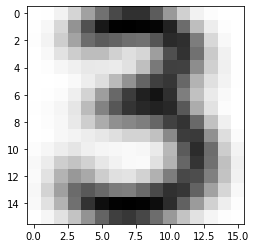
\includegraphics[width=\linewidth]{3_feature_1.png}
  \endminipage\hfill
  \minipage{0.25\textwidth}
    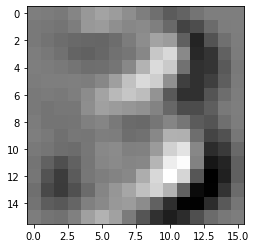
\includegraphics[width=\linewidth]{3_feature_2.png}
  \endminipage\hfill
  \minipage{0.25\textwidth}
  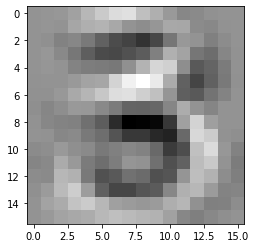
\includegraphics[width=\linewidth]{3_feature_3.png}
  \endminipage\hfill
  \minipage{0.25\textwidth}
  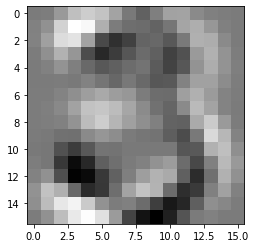
\includegraphics[width=\linewidth]{3_feature_4.png}
  \endminipage\hfill
  \caption{Examples of the first 4 columns of $U_3$.}
  \label{fig:3_feature}
\end{figure}

In order to classify unknown samples, a notion of distance, between that sample and the vector space representation of digits is needed.
So, when receiving the unknown sample, the algorithm porjects it onto the spaces of digits and compute the distance between the original sample and its projections.
At the end, the class with the smaller distance, with respect to the sample, is chosen as the predicted one.

Sample projection would be computed as $\vec{y}^\parallel=U(U^TU)^{-1}U^T\vec{y}$, but because the $(u_1,...,u_r)$ are ONB it simplifies to
\begin{equation}
  \vec{y}^\parallel_i=U_iU^T_i\vec{y}
\end{equation}

At the end, the distance $d_i=\|\vec{y}-\vec{y}^\parallel_i\|$ is computed for each class $i$ and the chosen one is 
\begin{equation}
pred\_class=\argmin_i (d_1,...d_n)
\end{equation}

All this reasoning applies to both the binary and multiclass classification task.

\chapter{Exercise 1 - Binary classification}\label{chap:ex1}
This exercise consists of a binary classification task, at first on digits 3 and 4, and then experimenting with different digit is required.
\ref{fig:3_4_instances} shows instances of digits 3 and 4 in the dataset.

\begin{figure}[!htb]
  \minipage{0.25\textwidth}
    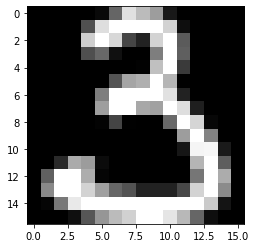
\includegraphics[width=\linewidth]{3_1.png}
  \endminipage\hfill
  \minipage{0.25\textwidth}
    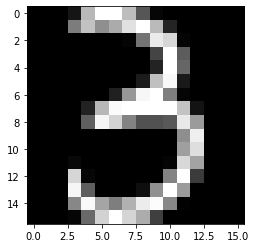
\includegraphics[width=\linewidth]{3_2.png}
  \endminipage\hfill
  \minipage{0.25\textwidth}
  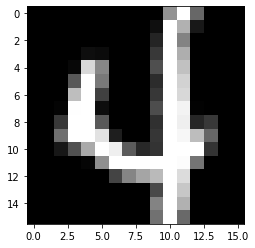
\includegraphics[width=\linewidth]{4_1.png}
  \endminipage\hfill
  \minipage{0.25\textwidth}
  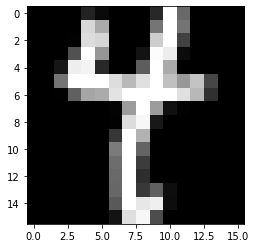
\includegraphics[width=\linewidth]{4_2.png}
  \endminipage\hfill
  \caption{Instances of digits 3 and 4 in the dataset.}
  \label{fig:3_4_instances}
\end{figure}

The procedure is:
\begin{itemize}
  \item load the dataset and the true class labels
  \item split them into training and test set (to do this I have used the function \emph{train_test_split} from \emph{sci-kit learn} with a 80\% training set)
  \item extract the training and test partitions relative to digits 3 and 4
  \item compute the SVD decomposition for each digit $X_i = U_i\Sigma_i V^T_i$, where $i=3,4$
  \item for each unknown sample from the test set compute its projection onto the spaces spanned by the relative columns of $U_3$ and $U_4$
  \item compute the distances between the projections and the original vector and choose as predicted class the one that minimize that distance
\end{itemize}
The evaluation metrics for this classifier are the misclassification error and the confusion matrix. 
As shown below, this classifier has a 0\% misclassified samples in case of digits 3 and 4.

\begin{figure}[h]
  \center
  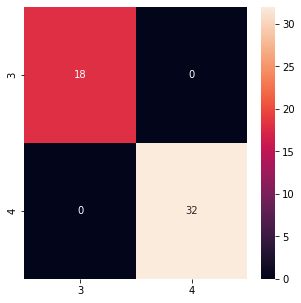
\includegraphics[width=0.45\linewidth]{3_4_cm.png}
  \caption{Confusion matrix for digits 3 and 4.}
  \label{fig:3_4_cm}
\end{figure}

Other experiments have been run over different combination of digits in order to investigate if visual similarity affects classification.
In particular, pairs tested are (3,8), (3,5), (6,9), (1,7).
Figure \ref{fig:binary_cls_mse} shows the results, while comments are reported in \ref{chap:conclusion}.

\begin{figure}[h]
  \center
  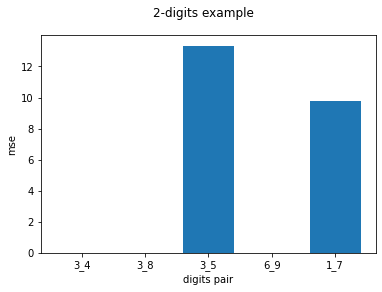
\includegraphics[width=0.45\linewidth]{binary_cls_mse.png}
  \caption{Misclassification error.}
  \label{fig:binary_cls_mse}
\end{figure}

\begin{figure}[!htb]
  \minipage{0.4\textwidth}
    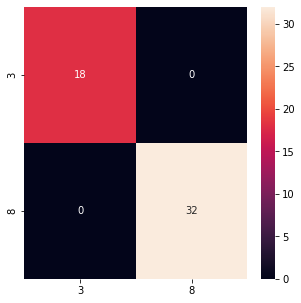
\includegraphics[width=\linewidth]{3_8_cm.png}
  \endminipage\hfill
  \minipage{0.4\textwidth}
    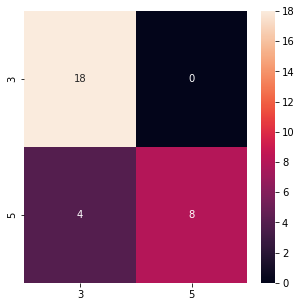
\includegraphics[width=\linewidth]{3_5_cm.png}
  \endminipage\hfill

  \minipage{0.4\textwidth}
  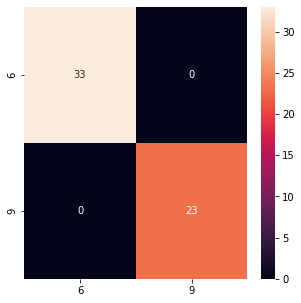
\includegraphics[width=\linewidth]{6_9_cm.png}
  \endminipage\hfill
  \minipage{0.4\textwidth}
  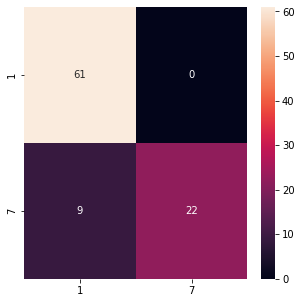
\includegraphics[width=\linewidth]{1_7_cm.png}
  \endminipage\hfill
  \caption{Confusion matrices for different experiments.}
  \label{fig:binary_cls_cm_2}
\end{figure}

\chapter{Exercise 2 - Multiclass Classification}\label{chap:ex2}
In the second exercise the problem of multinomial classification is addressed by generalizing the binary classifier of the previous exercise to the case of k different classes.
The algorithm is exactly the same as before.
Here I followed the idea to take the pairs tested in the previous exercise, add a new digit and observe how the distribution of predictions change relatively to the visual similarity.
\begin{figure}[h]
  \center
  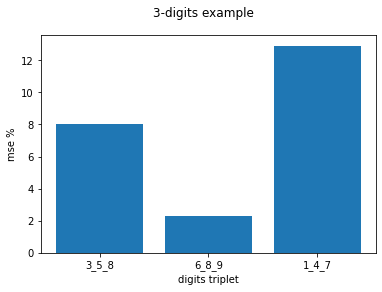
\includegraphics[width=0.45\linewidth]{multiclass_cls_mse.png}
  \caption{Misclassification error.}
  \label{fig:multiclass_cls_mse}
\end{figure}

\begin{figure}[!htb]
  \minipage{0.32\textwidth}
    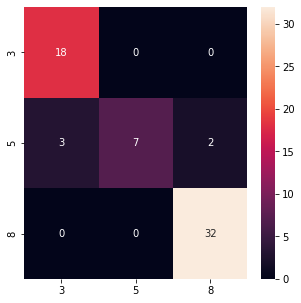
\includegraphics[width=\linewidth]{3_5_8_cm.png}
  \endminipage\hfill
  \minipage{0.32\textwidth}
  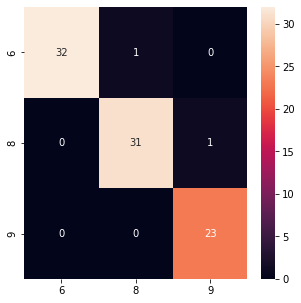
\includegraphics[width=\linewidth]{6_8_9_cm.png}
  \endminipage\hfill
  \minipage{0.32\textwidth}
  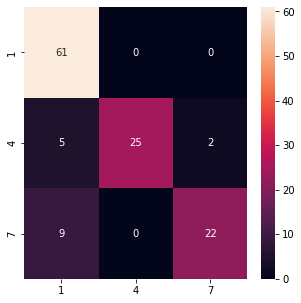
\includegraphics[width=\linewidth]{1_4_7_cm.png}
  \endminipage\hfill
  \caption{Confusion matrices for different experiments.}
  \label{fig:multiclass_cls_cm_2}
\end{figure}

\chapter{Conclusion}\label{chap:conclusion}
It is clear that a classifier based on SVD decomposition technique can perform very well on an "easy" task like digit recognition.

What is interesting is that visual similarity affects classification but only when also orientation is taken into account, at least for the 2- and 3-digits case: 
indeed, digits like 6 and 9, that from a human point of view could be judged "similar", differing only for a rotation factor, are well classified. 
Instead, digits like 1, 4 and 7, similar and with the same orientation, show a small, but non zero, classification error.

I tried to see if adding the digit 4 to the pair (1,7) could move some wrong prediction from 1 to 4 but it didn't happened.
My idea is that the more the complexity of the digit, in terms of strokes and angles, the more the chance to fail the classification: 
indeed, the classification errors for the digit 7 are all in favour of the digit 1 (less complex) and never in favour of digit 4 (more complex).
For the same reason, error classification for digit 4 are spread between digit 1 and 7.

Just for curiosity, I have implemented a general version of the classifier independent on the number of input digits. 
Results in \ref{fig:k_multiclass_cls_mse} and \ref{fig:multiclass_cls_cm_k} show that when all the digit, from 0 to 9, are included, the misclassification error reaches 60\% and the vast majority of errors is in favour of 0 digit.
I think this is due to the variance of shape when hand-writing digit 0: it is easy to draw shapes that share traits with other hand-written digits (example in \ref{fig:digits}).
Indeed, when dropping digit 0 the misclassification error falls from 60\% to around 24\% and prediction are more spread in the confusion matrix.
\begin{figure}[h]
  \center
  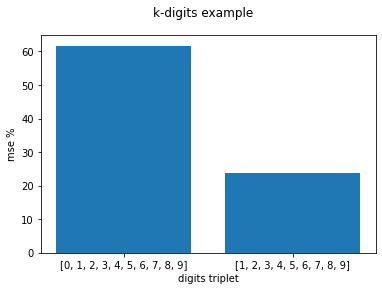
\includegraphics[width=0.45\linewidth]{k_multiclass_cls_mse.png}
  \caption{Misclassification error.}
  \label{fig:k_multiclass_cls_mse}
\end{figure}

\begin{figure}[!htb]
  \minipage{0.4\textwidth}
    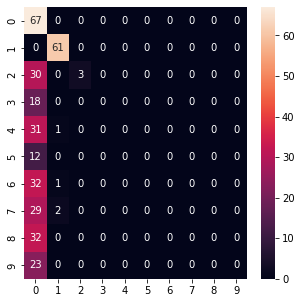
\includegraphics[width=\linewidth]{all_cm.png}
  \endminipage\hfill
  \minipage{0.4\textwidth}
  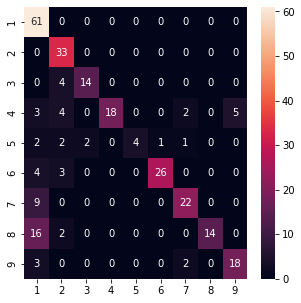
\includegraphics[width=\linewidth]{all_but_0_cm.png}
  \endminipage\hfill
  \caption{Confusion matrices for k-classifier with and without digit 0.}
  \label{fig:multiclass_cls_cm_k}
\end{figure}

\begin{figure}[!htb]
  \minipage{0.25\textwidth}
    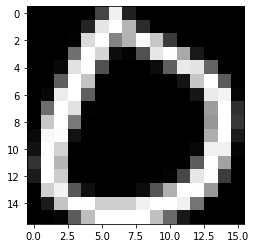
\includegraphics[width=\linewidth]{0.png}
  \endminipage\hfill
  \minipage{0.25\textwidth}
  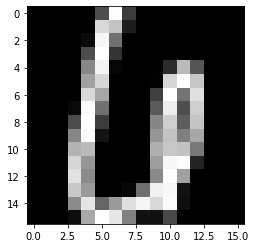
\includegraphics[width=\linewidth]{6.png}
  \endminipage\hfill
  \minipage{0.25\textwidth}
  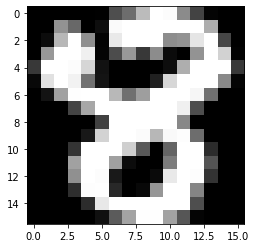
\includegraphics[width=\linewidth]{8.png}
  \endminipage\hfill
  \minipage{0.25\textwidth}
  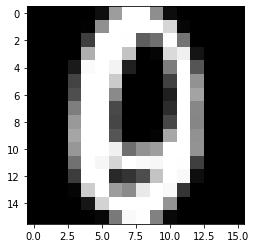
\includegraphics[width=\linewidth]{0_2.png}
  \endminipage\hfill
  \caption{Visual similarity between different digits.}
  \label{fig:digits}
\end{figure}
To conclude, SVD decomposition technique seems very powerful but also very sensitive to visual similarity. Neural network technique, although way more complex, have been proved to be very effective on this task reaching accuracies around 99\%.
\end{document}
